\documentclass[a4paper, 11pt]{report}

\usepackage{shorttoc}
\usepackage{amsmath}
\usepackage{amssymb}
\usepackage{graphicx}

\begin{document}

\begin{titlepage}
    %--------------------------
    % Page de garde du rapport
    %--------------------------
    \parindent=0pt

    \begin{minipage}{\linewidth}
        \begin{center}
        
\includegraphics[scale=0.28]{logo-lille1-2014.png}
        \end{center}
    \end{minipage}

    \vspace{0.4cm}

    \begin{minipage}{\linewidth}
        \begin{center}
        
\includegraphics[scale=0.28]{ESRF_logo.png}
        \end{center}
    \end{minipage}

    \vspace{0.4cm}

    \hrulefill
    \begin{center}\bfseries\Huge
        Modeling of protein shapes from SAXS data
    \end{center}

    \hrulefill
    \vspace*{1cm}
    \begin{center}\bfseries\Large           %author
        Guillaume Bonamis
    \end{center}

    \begin{center}\bfseries\Large           %supervisor
        Supervisor: J\'er\^ome Kieffer\\
        University tutor: Emeline Dudognon
    \end{center}

    \vspace*{\stretch{2}}
    \begin{flushright}
        August 27, 2015
    \end{flushright}   
    
    %rajouter un mot sur le tuteur Lille1
\end{titlepage}


\chapter*{Acknowledgements}
\addcontentsline{toc}{chapter}{Acknowledgements}
\pagenumbering{Roman}
    %-------------------------------------
    % Page pour les divers remerciements
    %-------------------------------------

I would like to thank my supervisor J\'er\^ome Kieffer for his help 
and his teaching all along my traineeship at the ESRF, my university 
tutor Emeline Dudognon for the time she spend to help me for my 
traineeship, Claudio Ferrero, head of ESRF Data Analysis Unit, for the 
revision of this report, Pierre Paleo, Thomas Vincent and Frederic 
Sulzmann for the numerous pieces of advice they gave me.


\tableofcontents
\addcontentsline{toc}{chapter}{Table of contents}


\chapter{Introduction}
\pagenumbering{arabic}
    %-------------------
    % Premier chapitre   
    %-------------------


\section{ESRF - The European Synchrotron}

The ESRF is a user facility providing with very intense X-ray beams to 
scientists to perform absorption, diffraction or spectroscopy 
experiments. 
The X-rays in a synchrotron are generated by electrons travelling at 
99.9999\% of the speed of light, inside a long, circular tube in nearly 
perfect vacuum.\\

At the ESRF, these electrons are first accelerated by a 16-metre-long 
linear accelerator (linac) before entering a small, racetrack shaped 
booster accelerator. 
Once they have reached their final speed (at an energy level of 6 GeV), 
these high-energy electrons are injected into the vacuum tube of the
844-metre-long storage ring.
Here they are guided on their orbital path by magnets. 
Between these magnets, the electrons pass through insertion 
devices, called undulators.
During each passage, the electrons release bursts of intense X-rays, 
along with electromagnetic radiation with other wavelengths, from 
infrared light to gamma rays. 
The X-ray bursts are projected in the forward direction, thin as a 
human hair (0.1 mm diametre).\\

The synchrotron X-ray beam leaves the main storage ring at a point a 
few metres after the undulator (ID beamlines) or the bending magnet 
(BM beamlines). 
Undulators are placed at 30 positions around the storage ring.
When leaving the storage ring, the X-rays enter one of 41 beamlines, 
each an ensemble of laboratory blocks or “hutches” where the actual 
research takes place. 
Figure~\ref{fgr:synchrotron} summarises this.

\section{BioSAXS beamline BM29}
\label{bm29}
BM29 \cite{BM29paper} is a beamline for Small Angle X-ray Scattering 
(SAXS) experiments of biological macromolecule solutions with the goal 
of determining their 3-dimensional structures in a natural state with 
'low' resolution (a few nanometers). 

\begin{figure}
\centering
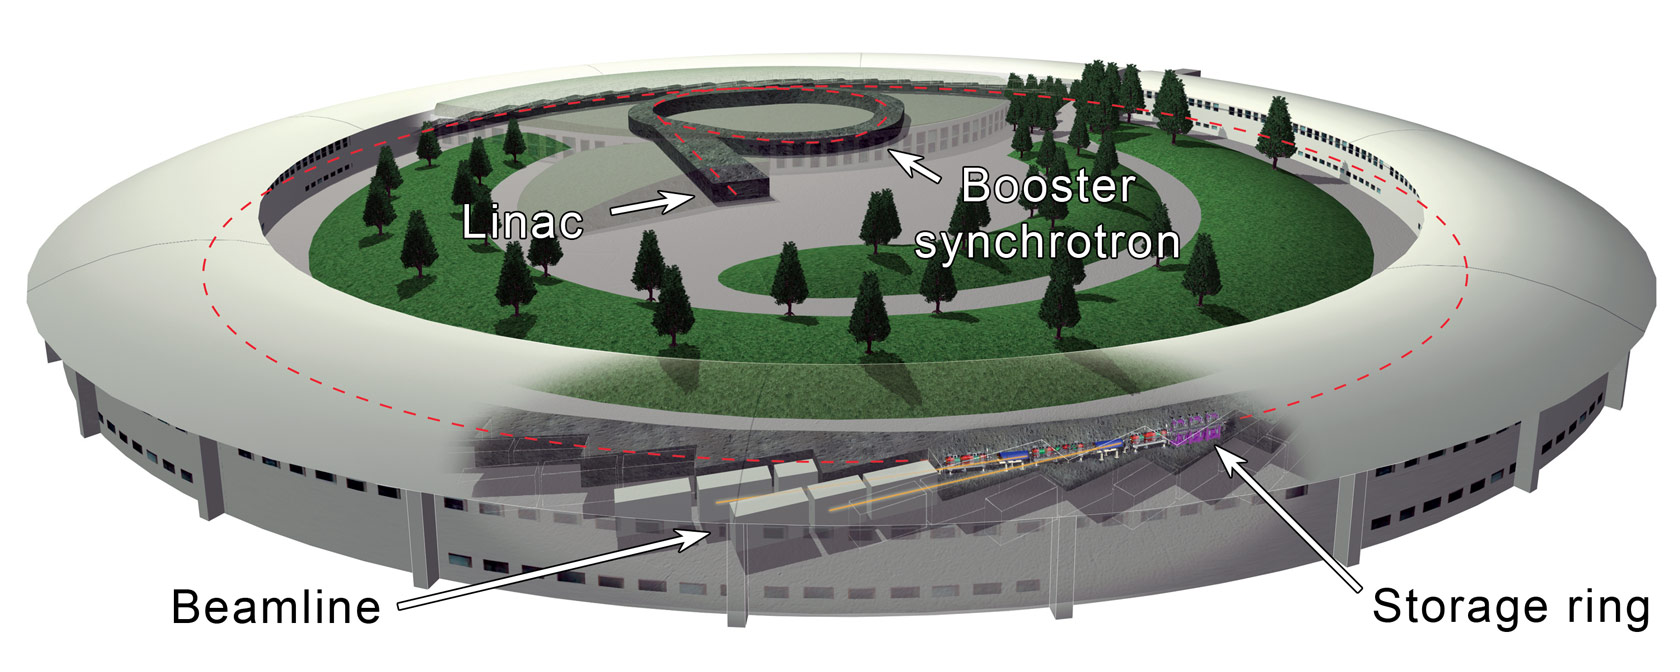
\includegraphics[scale=0.22]{synchrotron.png}
\caption{View of the ESRF with its main components, linac, booster, 
    storage ring and beamlines}
\label{fgr:synchrotron}
\end{figure}

The beamline data acquisition is based on a pipeline of individual 
tasks, highly automated, from the inputs to the final results. 
Here this series of process will be briefly described, focussing on 
what is relevant to our subject.
All data treatments have recently been described in \cite{BM29news} 
(submitted to \textit{Journal of Applied Crystallography}).

The series of tasks is controlled by EDNA, which is a plugin-based 
framework dedicated to data analysis pipelines \cite{edna}. 
It begins with the acquisition of the 2-D image of the pattern 
scattered from the studied sample, the detector being a Pilatus 1M for 
BM29. 
The global data-analysis process can be divided in four steps: 
\begin{itemize}
 \item azimuthal integration of the image
 \item background correction (scattering from the sample buffer)
 \item basic analysis of the scattering curves
 \item ab initio modeling
\end{itemize}

\begin{figure}
\centering
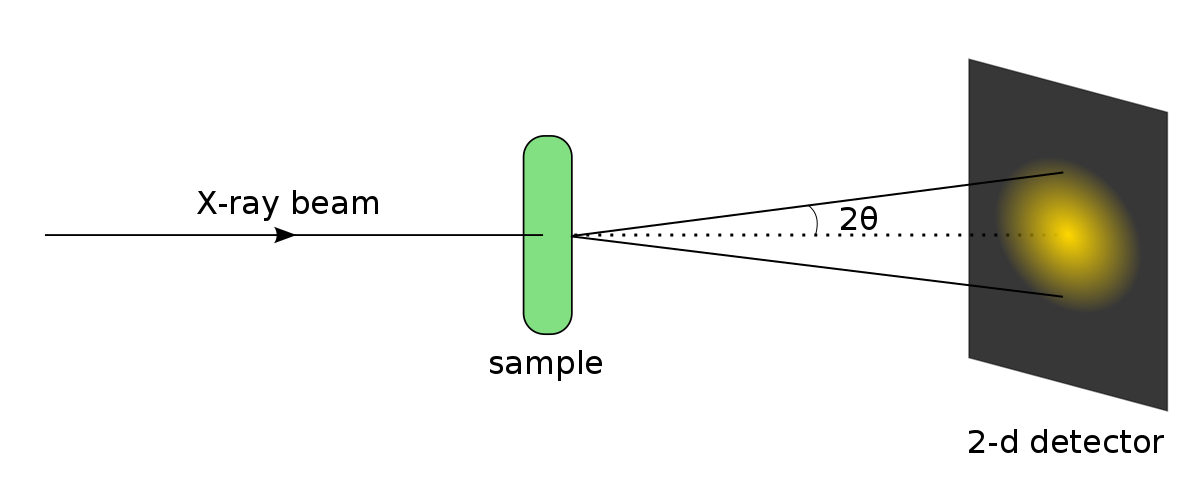
\includegraphics[scale=0.3]{schemaSAXS.png}
\caption{Schema of a SAXS experiment, scattering of the incident beam 
    creates the scattered image on the detector}
\label{fgr:schemaSAXS}
\end{figure}

The image obtained represents the X-ray scattering from the sample, it 
has a cylindrical symmetry along the incoming beam, as seen in 
figure~\ref{fgr:schemaSAXS}. 
The first step consists in averaging the 2-D image along the 
symmetry axis (azimuthal integration).  
This operation is performed using FabIO \cite{fabio} for image reading 
and PyFAI \cite{pyFAI} for the azimuthal integration. 
The result is a curve representing the scattered intensity as a 
function of the scattering vector $q = 4 \pi \frac{sin\theta}{\lambda}$ 
(expressed in inverse nanometres).

This curve has to be background corrected: an EDNA plugin subtracts the
background scattering intensity, recorded using a buffer
solution from the sample curve resulting in the sole scattering signal 
of the macromolecule. 
The background corrected curve is then analysed using several tools 
from the \textsc{atsas} package \cite{atsas}. 
The EDNA analysis pipeline generates automatically Guinier and Kratky
plots for visual analysis of the scattering signal.\\

The fourth step of the data analysis is the ab initio modeling, 
presented in the following section, which is the core of the subject.

\section{Ab initio modeling}
\label{modeling}                           %flag pour citer cette section

Ab initio modeling aims at building a low-resolution 3-D model of the 
macromolecule of interest. 
BM29 staff uses for this other tools from the \textsc{atsas} package 
as follows.\\

The first step of the modeling consist in reconstructing many ($N$, ususally 8
or 16) 3-D dummy-atom models (DAM) from the background corrected curve using 
\textit{dammif} \cite{dammif}. 
These DAM are then selected according to two parameters related to the 
curve: 
\[
R = \frac {\sum {||I_{obs}| - |I_{calc}||}}{\sum {|I_{obs}|}}; \ \ \ 
\chi^{2} = \sum {\frac {(I_{obs} - I_{calc})^{2}}{\sigma^{2}}}
\]
These two values allow evaluating the goodness of the fit. 
The thresholds are respectively the mean plus one or two standard 
deviations; models out of range are simply discarded.

The remaining DAM are then superimposed two by two using the 
\textit{supcomb} \cite{supcomb} program which reports the Normalized 
Spatial Discrepancy (NSD), a metric to evaluate the difference between 
two models. 
It allows the segregation of similar models from the others. 
Model outliers are discarded based on the NSD
values.
For each DAM, the mean of its NSD from others is computed; if the mean 
value exceeds the average plus twice the standard deviation, it is 
discarded. 
The DAM with the lowest average value is the reference model.

During the process, $N - n$ models remain and one of them is the 
reference ($n$ is the number of discarded models, due to $R-value$, 
$\chi^{2}$ and NSD). 
All these $N - n$ models are merged with \textit{damaver} 
\cite{damaver}. 
Subsequently \textit{damfilt} gets the average DAM (which is not solution of
the problem) and \textit{damstart} generates an input model for 
\textit{dammin} \cite{dammin} which refines the model to fit the 
background subtacted curve. 
The outcome of the Monte Carlo refinement performed by \textit{dammin} 
is the final model which can be interpreted by biologists (comparison 
with molecule fragments coming from Nuclear Magnetic Resonance or 
comparison with other techniques).

\section{Traineeship subject}

The task of the traineeship was to work on the part "superimposition 
and selection of the models" of the modeling process. 
In fact, the modeling process is the most problematic according to 
the beamline scientists for several reasons:
\begin{enumerate}
\item the BM29 pipeline is based on Python, whereas most
of the \textsc{atsas} package is written in Fortran, so for a better 
integration into the pipeline, a Python library could be advantageous. 
\item programs from this package are closed source and 
changing from version to version add difficulties to the process of 
their integration into the pipeline. 
\item the execution time of these programs causes the ab initio 
modeling to be the bottleneck of the BM29 pipeline. 
\item sometimes the whole EDNA pipeline needs to be aborted 
due to \textit{dammin}, not returning results after half an hour.
\end{enumerate}

In agreements with these observations, it was decided to create a 
homemade package to overcome these data analysis problems. 
This package has been called FreeSAS, is open source and free (under 
the MIT License). 
Written in Python, it aims at providing tools for the BioSAXS data 
analysis with an optimized execution time and providing reliable 
results. 
The main activity of my traineeship was around this Python package, 
and especially the re-implementation of the superimposition of the DAM 
(previously done by \textit{supcomb}) and the selection of these to 
continue the process.

In chapter 2, we will describe the whole implementation of FreeSAS, 
and the theory behind it, to reach our aim. 
Then, in chapter 3, we will present an application of FreeSAS using the 
scattering curve obtained from a protein called Lysozyme 
(figure~\ref{fgr:lysozyme}). 
\begin{figure}
\centering
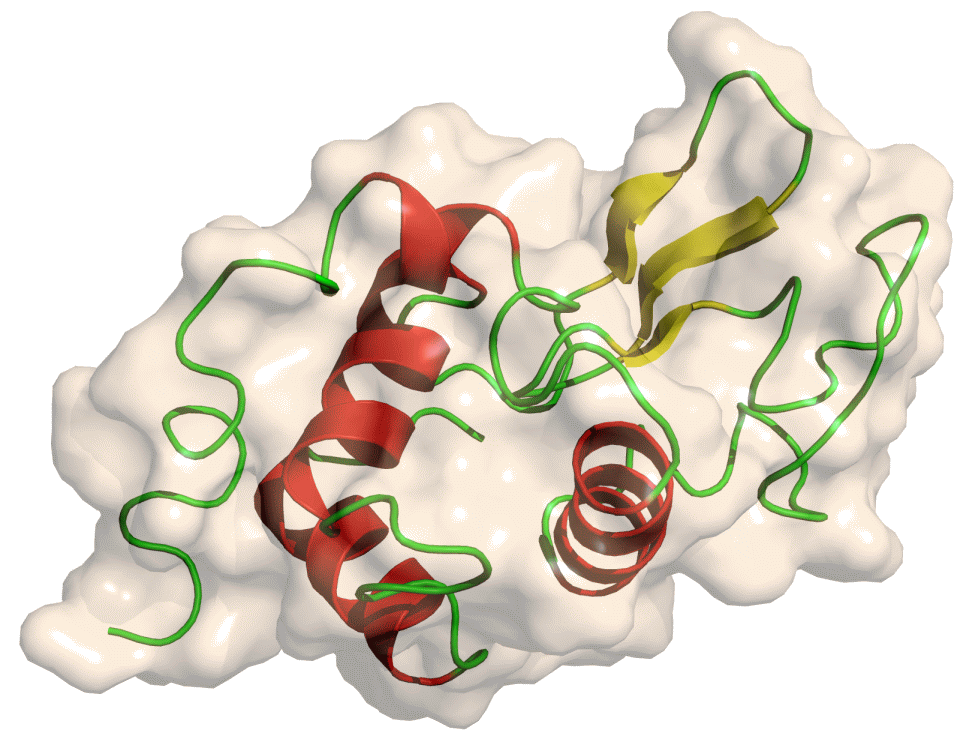
\includegraphics[scale=0.2]{lysozyme_wiki.png}
\caption{Lysozyme protein structure, high- and low-resolution (image 
  from Wikipedia)}
\label{fgr:lysozyme}
\end{figure}

We will use this protein all along the report for examples, 
presentation of results and code performances. 
This protein is very common in biology and simple to study. 
In particular, it is present in egg white. 
The scattering curve of lysozyme comes from \textsc{atsas}, which uses 
it for test purposes (figure~\ref{fgr:saxscurve}).

\begin{figure}
\centering
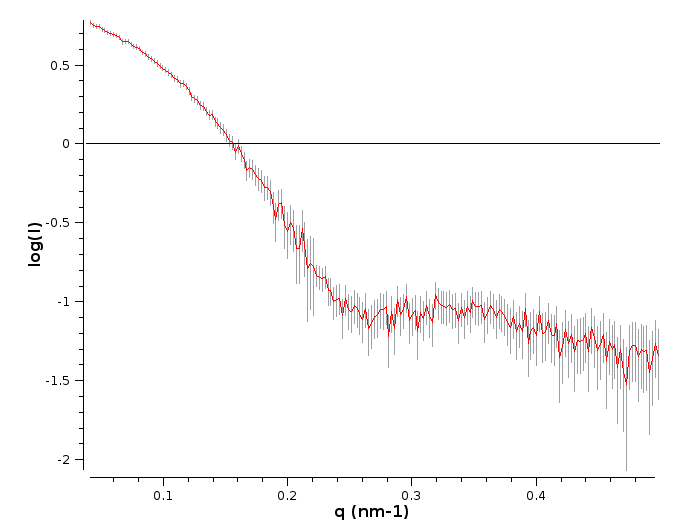
\includegraphics[scale=0.45]{saxscurve.png}
\caption{SAXS curve of the lysozyme protein provided in \textsc{atsas}}
\label{fgr:saxscurve}
\end{figure}


\chapter{FreeSAS implementation}
    %--------------------
    % Deuxieme chapitre  
    %--------------------
%\setcounter{page}{7}

FreeSAS is a Python package for BioSAXS data analysis. 
It is comprised of several modules, each focusing on a special task. 
We will describe, for each module of FreeSAS:
\begin{itemize}
 \item the tasks needed to be performed
 \item the physical theory behind the task and its usefulness in our 
       global process
 \item the different Python tools and algorithms used in the module to 
       perform task
\end{itemize}
The last section will describe the way all these tasks are exploited 
to create a "global process" computing the wanted result. 

\section{Reading input data}

The library has to be able to work within the BM29 pipeline presented 
in section \ref{bm29} and used in production for a few years  now. 
As a component of a larger piece of software, it has to deal with 
inputs coming from other software, especially the \textsc{atsas} 
programs used upstream and needs to provide outputs compatible with 
\textsc{atsas}, used also downstream. 
Here we will focus on the reading of the input structures and describe the
data we are interested in.

The inputs of the superimposition module are the DAM outputs of the 
various \textit{dammif} runs. 
These structures are written in files using the PDB format (Protein 
Data Bank) \cite{pdb}, a standard representation of macromolecular 
structure data.\\
The (simplistic) parser we have written copes with two things: reading 
the atoms' coordinates (beads) and retrieving the quality of the fit 
of the model on the experimental data ($\chi^2$ and $R$-value). 
These numbers represent the quality of the model and are calculated 
using the difference between the actual SAXS curve and the simulated 
one. 
These quality factors are used used to reject models badly reproducing 
experimental data.

The second piece of information to retrieve are the dummy atoms 
coordinates. 
These are not actual atoms, but they indicate that there is some 
material (the macromolecule) in their positions, and where there are 
no dummy atoms, it is solvent. 
Typical DAM used in this project had 500 dummy atoms (order of 
magnitude). 
The parser written was dedicated to the following task: read the PDB 
file to select the data needed, and then keep in memory on the one 
hand the $R-value$ of the DAM and on the other hand the Cartesian 
coordinates (x, y, z, in Angstrom) of each dummy atom of the model. 
These coordinates are stored as a 2-D numpy array from the 
\textit{NumPy} package \cite{numpy}; they are necessary for the 
geometric operation we will have to make along our process.

\section{Similarity calculations}

In order to be able to merge similar models, and reject dissimilar 
ones, one needs to define the similarity of two models. 
This section introduces a ``distance'' to measure this  
similarity and describes its implemention in the FreeSAS
package.

The likeness of two 3-D models can be, at a first glance, very 
subjective. 
To be able to compute it, we use the NSD metric, introduced by Kozin 
and Svergun in their paper \textit{Automated matching of high- and 
low-resolution structural models} \cite{supcomb}. 
This value quantifies the dissimilarity between two sets of 
point $S_{1}$ and $S_{2}$, in our case in a 3-D space.
These sets are neither ordered nor of the same size ($N_{1}$ points 
for $S_{1}$ and $N_{2}$ points for $S_{2}$), making unusable in our 
case other techniques like Kabsch method \cite{kabsch1976}.
NSD is analogous to the standard Euclidian distance, but as it is 
normalized, it is not homogeneous to a distance. 
The following formula defines the NSD:

\[
\rho(S_{1},S_{2})= \frac{1}{2} \sqrt {\frac{1}{N_{1}d_{2}^2} 
\cdot \sum\limits_{i=1}^{N_{1}} \rho^2(s_{1i}, S_{2}) + \frac{1}{N_{2}d_{1}^2} \cdot \sum\limits_{i=1}^{N_{2}} \rho^2(s_{2i}, S_{1})}
\]

For a point $s_{1i}$ in $S_{1}$, the Euclidian distance with all the 
points of $S_{2}$ is computed, and the minimal one is denoted as 
$\rho(s_{1i}, S_{2})$. 
The other parameters in the formula are the finenesses $d_{i}$. 
The fineness corresponds to the average Euclidian distance between a 
point of $S_{i}$ and its nearest neighbour.

The NSD can be used to measure the similarity of two sets of points as:
\begin{itemize}
 \item it is symmetric, $\rho(S_{1},S_{2}) = \rho(S_{2},S_{1})$
 \item it is stable, $\rho(S_{1},S_{2})$ function has a stable minimum
 \item $\rho(S_{1},S_{2}) = 0$ only if $S_{1} = S_{2}$
\end{itemize}

As the calculation of the NSD is the core of our process, it is of 
primary importance to optimize its implementation. This has been 
optimized in 3 subsequent steps (and supervised by careful profiling):
\begin{enumerate}
  \item Numpy implementation calculating the 2-D table of distances from all
  atoms in $S_{1}$ to any atom in $S_{2}$, performing subsequently the search 
  of the minimum in each row and column.
  \item Cython implementation \cite{cython} (a kind of Python code translated
  to C) which performs simulatneously the searches for a minimum (along row 
  and column) for each pair of atoms, preventing a large 2-D array allocation.
  \item An OpenMP \cite{openmp} implementation of the Cython version taking
  benefit from the multi-core systems available on modern computers.
\end{enumerate}

\section{Coarse superimposition of models}

The DAM, as generated by \textit{dammif}, are randomly oriented, so the NSD
between two models is not representative of their similarity.
That is why we have to first superimpose the models, using 
translation, rotation and symmetry operations, so that the NSD only 
points out the dissimilarity.\\

The strategy implemented to superimpose two DAM (sets of
dummy atoms $S_{1}$ and $S_{2}$) is similar to the one described in 
Kozin and Svergun's publication \cite{supcomb} and goes via a three 
steps process to bring them into their canonical position:
\begin{itemize}
  \item the center of mass of the model is at the origin of the 
        coordinate axes (canonical translation)
  \item the principle axes of inertia of the model are aligned along 
        the coordinate axes (canonical rotation)
\end{itemize}
The last step consists in applying a special symmetry operator to 
$S_{2}$ to select the enantiomorph of $S_{2}$ corresponding to the one 
of $S_{1}$ (enantiomorph selection).

We will illustrate this process showing the NSD between two models 
after each step. 
To this effect, we will use two models generated by \textit{dammif} 
from the lysozyme scattering curve. 
The 3-D structures of both models after each step are presented in 
appendix~\ref{alignstep}.
The initial NSD between the two models is $1.01$.

\subsection{Canonical translation}

The first stage consists in superimposing the center of mass (COM) of 
the two models. 
In the dummy atom model, all the dummy atoms have the same mass so the 
COM coordinates of the model $k$ are computed as follow:
\[
x_{k}^0 = \frac{1}{N_{k}} \cdot \sum\limits_{i=1}^{N_{k}} x_{ik};\ \ \ 
y_{k}^0 = \frac{1}{N_{k}} \cdot \sum\limits_{i=1}^{N_{k}} y_{ik};\ \ \ 
z_{k}^0 = \frac{1}{N_{k}} \cdot \sum\limits_{i=1}^{N_{k}} z_{ik}
\]\\
The canonical translation to send the model $S_{k}$ to the coordinates' 
origin is calculated with $(-x_{k}^0,\ -y_{k}^0,\ -z_{k}^0)$ vector to 
obtain the $4 \time 4$ canonical translation matrix of $S_{k}$: 
$T_{k}^0$.

With both models translated to their center of mass, the NSD between 
the two lysozyme DAM is $1.00$. 
The improvement is really modest because the initial COM of each model 
are already close to one another.

\subsection{Canonical rotation}

The next step is the alignment stage. 
To compute the canonical rotation matrix of $S_{k}$, which will align 
the principle axes of inertia of $S_{k}$ with the coordinates' axes, 
we first need to know its inertia tensor. 
This has to be computed using the COM of $S_{k}$ at the coordinates 
origin. 
The inertia tensor is given by:
\[
I_{k}=
\begin{pmatrix}
 I_{11} & I_{12} & I_{13} \\
 I_{21} & I_{22} & I_{23} \\
 I_{31} & I_{32} & I_{33} \\
\end{pmatrix}
\]\\
and knowing that each point of the set $S_{k}$ is defined by
$
s_{kq}=
\begin{pmatrix}
 x_{kq}^1 \\
 x_{kq}^2 \\
 x_{kq}^3 \\
\end{pmatrix}
$\\
we have, with $\delta_{ij}$ the Kronecker delta,
\[
(I_{k})_{ij} = \frac{1}{N_{k}} \cdot \sum\limits_{q=1}^{N_{k}} 
[\delta_{ij} \cdot \sum\limits_{l=1}^3 
 (x_{kq}^l - {x_{kq}^l}^0)^2 -  (x_{kq}^i - {x_{kq}^i}^0) 
 \cdot (x_{kq}^j - {x_{kq}^j}^0)]
\]\\
It appears that the $I_{k}$ tensor is symmetric real, hence we know 
that it can be diagonalized; we can compute its three eigenvalues 
$\lambda_{k1} \geq \lambda_{k2} \geq \lambda_{k3}$ and the three 
eigenvectors corresponding $v_{k1},\ v_{k2},\ v_{k3}$. 
We can create a rotation matrix composed by the eigenvectors of 
$I_{k}$, arranged in columns and sorted in increasing order of the 
associated eigenvalues. 
If this matrix is named $M_{k}$, its transposed $[M_{k}]^T$ is the 
rotation matrix which align $S_{k}$ axes of inertia along the 
coordinates axes \cite{supcomb}, i.e. the one we are looking for 
($4 \time 4$ rotation matrix).

Including the canonical rotations for each models to the process, we 
obtain a NSD value between the two DAM of $0.60$ (before it was 
$NSD = 1.00$).

\subsection{Enantiomorph selection}

Before being able to superimpose correctly $S_{2}$ on $S_{1}$, we need 
to take into account enantiomorphs. 
In fact, two enantiomorphs of a macromolecule generate the same SAXS 
curve, so that this method does not allow to distinguish them. 
This means that we do not make a difference for our data analysis 
between two enantiomorphs.
But this operation needs to be implemented. 
As we superimpose $S_{2}$ on $S_{1}$, we will force $S_{2}$ to be in 
the same enantiomorphic form as $S_{1}$. 
For this purpose, we have to set $S_{1}$ and $S_{2}$ in their canonical 
positions, i.e. apply to them the transformation 
$[M_{k}]^T \times T_{k}^0$ ($\times$ is here the matricial product).

Eight transformations are then performed on $S_{2}$ which correspond 
to the eight possible symmetries, four for each enantiomorph. 
Transformation matrices are as follow:
\[
\begin{pmatrix}
 \pm 1 & 0 & 0 & 0 \\
 0 & \pm 1 & 0 & 0 \\
 0 & 0 & \pm 1 & 0 \\
 0 & 0 & 0 & 1
\end{pmatrix}
\]\\
After each transformation, the NSD between $S_{1}$ and $S_{2}$ is 
computed. 
The one minimizing the NSD is kept as the good symmetry for the 
subsequent steps. 
The rotation matrix for $S_{2}$ is now the product of the previous 
one, $[M_{2}]^T$, by the symmetry matrix, and we will call it 
$R_{2}$.\\

Finally, we are able to compute for a set of dummy atoms $S_{k}$ the 
canonical translation and rotation matrices. 
We know also the transformation to apply to force a DAM to be in the 
same enantiomorphic form as the other one. 
To canonically superimpose two DAM we can apply on them the required 
transformation but we chose to align always the second DAM on the 
initial position of the first one (to save execution time).\\
Thus, we apply the following transformation to $S_{2}$:
\[(T_{1}^0)^{-1} \times M_{1} \times R_{2} \times T_{2}^0\]

At the end of this process, we have two DAM whose centers of mass and 
principle axes of inertia are superimposed (canonical superimposition). 
In our example, we obtain after this process a NSD equal to $0.58$.

After this coarse superimposition process, the NSD between the two DAM 
decreased from a $NSD_{init} = 1.01$ to $NSD_{final} = 0.58$. 

\section{Refined superimposition}

The canonical superimposition produces a good fit of the two models 
(if they are similar), but the alignment remains coarse, we need to 
optimize the superimposition to better characterize the dissimilarity 
between two DAM. 
The core of the superimposition process remains the same, we will add 
to it the following refinement algorithm.\\
 
We have to optimize the transformation applied to $S_{2}$ to align it 
with $S_{1}$, and the criterion of improvement will be the NSD, which 
has to be as low as possible. 
To this effect, we use the simplex optimizer provided by the 
\textit{SciPy} library \cite{scipy}, but to use it, accurate numerical 
parameters are needed. 
What we did was to extract from the global transformation matrix 
six transformation parameters: 
$(x_{0}, y_{0}, z_{0})$, 
corresponding to the total translation applied to $S_{2}$, and 
$(\alpha,\ \beta,\ \gamma)$, 
which are the Euler angles of the total rotation. 
The optimizer reads in these six parameters and calls a function which 
returns the NSD between $S_{1}$ and $S_{2}$ after the input 
transformation has been applied to $S_{2}$. 
This call is repeated, refining each time the six parameters values to 
minimize the NSD.

The optimizer is stopped when convergence has been reached and returns 
the six refined parameters and the minimized NSD. 
The final NSD value is assumed to reflect the actual dissimilarity 
between them.\\

If we add to the coarse superposition this refinement process we 
obtain $NSD_{refined} = 0.51$ in the example of the two lysozyme DAM. 
We can conclude that the refinement provides a significant improvement 
of the superimposition (from $0.58$ to $0.51$), however the coarse 
superimposition has already yielded a good approximation (from $1.01$ 
to $0.58$).

\section{Dummy atom models selection}

The algorithm superimposing two DAM was implemented in order to 
superpose the $N$ models generated by \textit{dammif}.\\

For it, \textit{dammif} PDB files are first read in through the 
FreeSAS parser and relevant data are extracted. 
Some properties are then computed from it (COM, inertia tensor,...). 
At this stage we have $N$ detailed DAM and all we need is to 
superpose them.

The superposition is implemented to obtain a $N \times N$ NSD table. 
We want a $N \times N$ table with 
\[
table_{ij}=NSD(S_{i},S_{j})
\]\\ 
We know that we have zeros on the diagonal and that the table is 
symmetric because of the two properties of the NSD:
\[
NSD(S_{i},S_{i})=0.00 \Rightarrow table_{ii}=0.00
\]
\[
NSD(S_{i},S_{j}) = NSD(S_{j},S_{i}) \Rightarrow table_{ij}=table_{ji}
\]\\
As a consequence, we can compute $\frac{N \cdot (N-1)}{2}$ optimized 
superpositions instead of $N \times N$.\\

Once the NSD table is generated, we have all what we need to select 
the dummy atom models.\\
The first selection criteria have already been presented in 
section~\ref{modeling}: the $\chi^2$ and the $R-value$. 
These two parameters are not dependent on the DAM positions as they 
are computed before any movements. 
For gaining execution time, the tests on them are performed before 
the superposition process, thus some models (say $m$) are discarded 
before being superimposed, allowing skipping superposition 
optimization steps to save time: $\frac{(N-m) \cdot (N-m-1)}{2}$ 
instead of $\frac{N \cdot (N-1)}{2}$.

Next the average NSD between each model and the others is computed 
(section\ref{modeling}) using the NSD table and the test is performed 
for each remaining DAM ($N-m$ at this stage). 
A new series of models is discarded (or not), that give us the 
$N-n$ acceptable DAM to follow the modeling process of EDNA. 
Moreover, the model with the lowest average NSD is set as "reference 
model".\\

At the end of this procedure, data are formatted to present 
consistently the analysis results. 
First, the DAM is saved using the PDB format to be accessible to 
the next program in the pipeline: \textit{damaver}. 
The models are aligned on the reference one and are saved in this 
configuration, as needed by \textit{damaver}. 
Information about the selection process is also saved for the BM29 
users. 
A piece of code has been written to create figures with $\chi^2$ and 
$R-value$ and respective thresholds, the NSD table and the average NSD 
values and related threshold. 
These figures are generated using the \textit{matplotlib} Python 
library \cite{matplotlib}.\\

It should be noted that FreeSAS provides tools to read data from PDB 
files and to process them using several algorithms. 
At the end, it returns the target DAM ready to be used by 
\textit{damaver} along with all data which might help the users in 
their analysis.

We will see in chapter 3 an example of usage of the FreeSAS package 
with data from a SAXS experiment on lysozyme.


\chapter{Lysozyme modeling with FreeSAS}%titre ???
    %---------------------
    % Troisieme chapitre  
    %---------------------

In this chapter we will present some results obtained using FreeSAS 
tools analyzing lysozyme.

Firstly the program used for this data treatment will be described. 
Then, the results returned by this program will be presented. 
In the end our program's performances will be compared with those of 
the \textsc{atsas} package.

\section{SuPyComb script}

The tools from FreeSAS have been integrated into the pipeline of BM29 
\cite{BM29news}, but are also available as a stand-alone program: 
\textit{SuPyComb}.\\

The program source is written in Python and takes PDB files from 
\textit{dammif} as arguments. 
It carries out the selection according to the $R-value$, the 
superposition of the $N$ dummy atom models, the selection based on the 
NSD mean, the selection of the reference model and the alignment of 
all valid models on the reference one.\\
\textit{SuPyComb} can be run in two different ways, depending on the 
number of input models:
\begin{itemize}
  \item if there are only two models, the second one is simply 
        superimposed on the first one as presented in chapter 2.
        \textit{SuPyComb} returns the final NSD value and a PDB file 
        with the coordinates of the second model aligned on the first one.
  \item if there are more than two models, \textit{SuPyComb} carries out 
        selections and superimposition as mentionned above. 
        It returns the $N \times N$ NSD table, a graph with the $R-values$, 
        the maximal accepted value and the average NSD with all the other 
        models and its threshold for each DAM.
\end{itemize}
Moreover, some options are available for \textit{SuPyComb} users, and 
especially these ones:
\begin{itemize}
  \item Slow mode / fast mode:
  For the slow mode, the optimization of the NSD is done for each symmetry 
  (i.e. 8 times) whereas for the fast mode, the best symmetry is first 
  choosen without optimization and only the NSD for this symmetry is 
  optimized.
  The result is that the slow mode is nearly 8 times slower than the fast 
  one.
  \item Enantiomorph option:
  This option can be used in order for the program to look up or not 
  enantiomorphs. 
  If not, the program will not test 8 symmetries but only 4. 
  Thus, it will not be able to recognize two enantiomorphs of the 
  same protein.
\end{itemize}

\section{Results of the lysozyme study}%TODO revoir le titre

We took the scattering curve of lysozyme as an argument for 
\textit{dammif}, that we ran 16 times in its slow mode. 
Thus, we obtain 16 PDB files containing data for 16 dummy atom models 
of nearly 3000 dummy atom each.\\

We ran \textit{SuPyComb} with these 16 files as arguments in fast mode 
and with the enantiomorphs search option. 
One output is the graph presented in figure~\ref{fgr:rfactor}. 
\begin{figure}
\centering
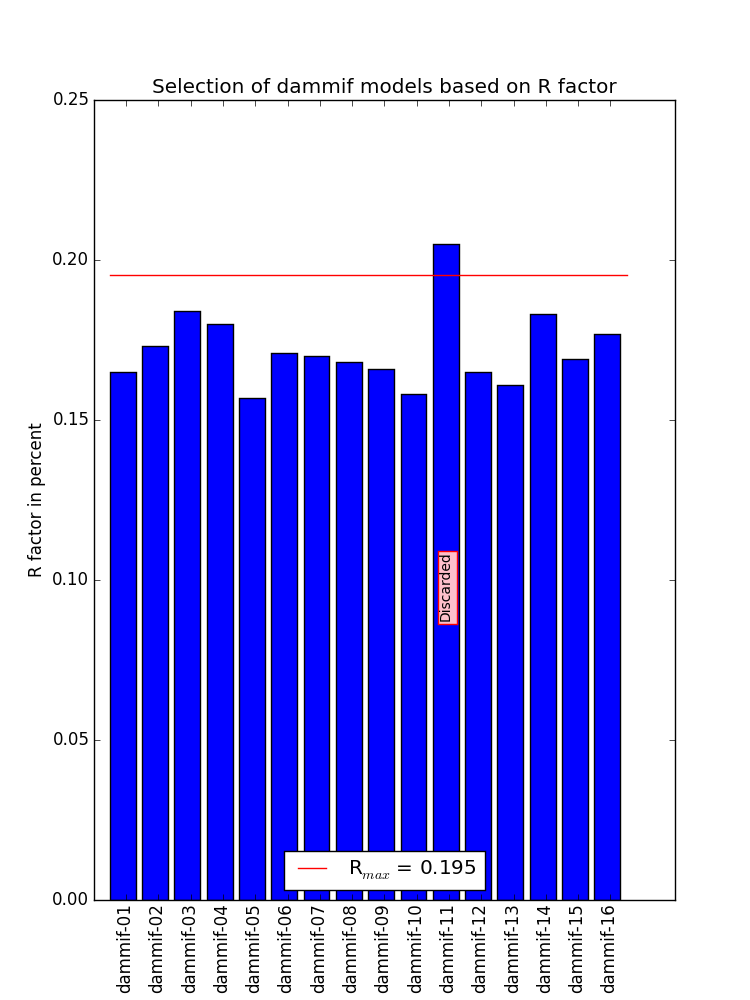
\includegraphics[scale=0.6]{Rfactor.png}
\caption{Graph showing the $R-value$ of each DAM, the threshold $R_{max}$ 
         and the discarded DAM}
\label{fgr:rfactor}
\end{figure}
It points out the fact that the $R-value$ of one of the models 
("dammif-11") exceeds $R_{max}$, which is the average of the 
$R-values$ plus twice the standard deviation. 
The DAM "dammif-11" is automatically flagged as non-valid and is 
discarded. 
The model will not taking into account in the subsequent 
\textit{SuPyComb} process that will save execution time.

After the whole process detailed in chapter 2, \textit{SuPyComb} 
returns the two graphs presented in figure~\ref{fgr:nsd}. 
\begin{figure}
\centering
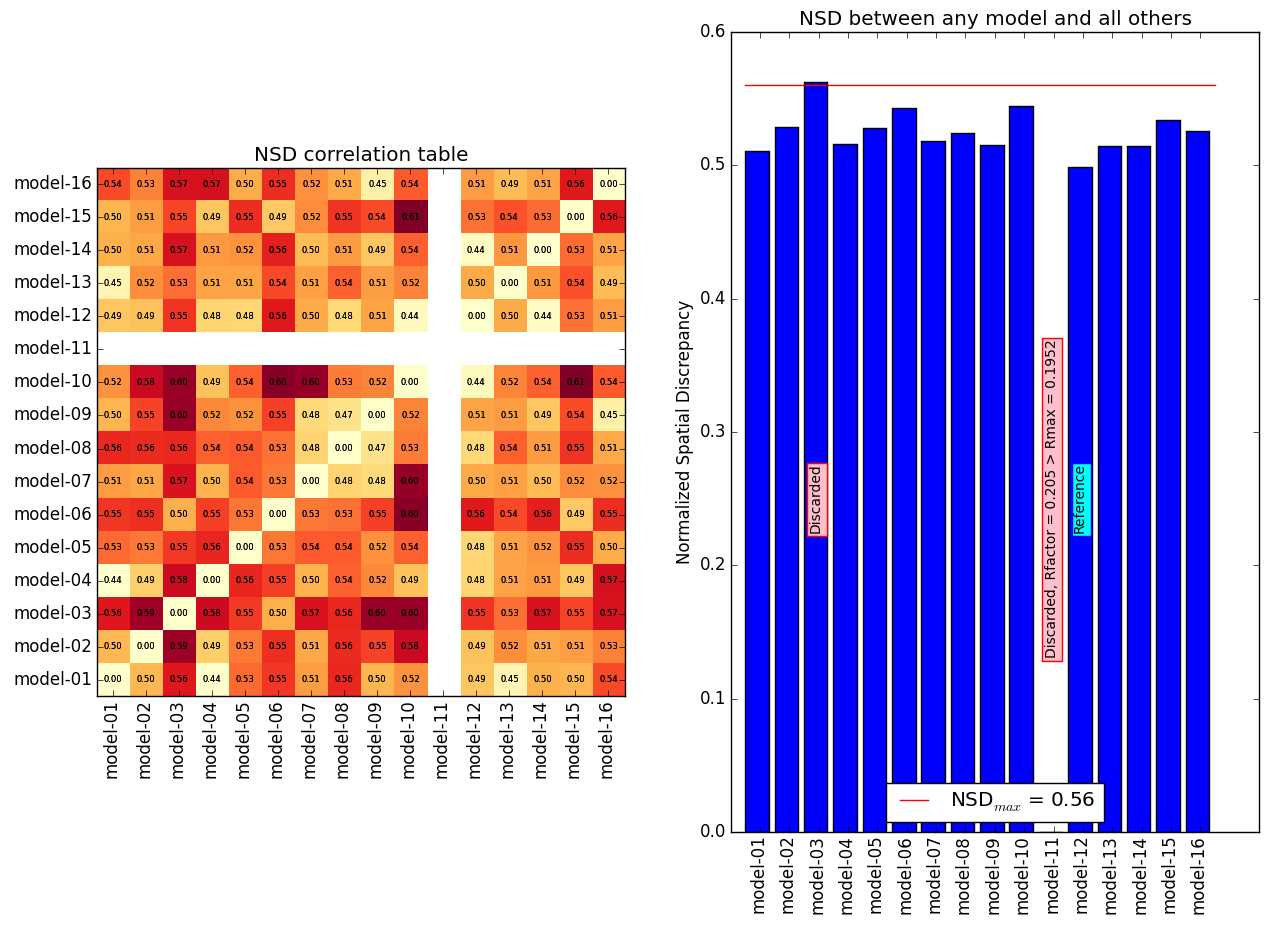
\includegraphics[scale=0.45]{nsd.png}
\caption{Two graphs computed by \textit{SuPyComb}, the NSD table and 
         for each model the average NSD with all the others}
\label{fgr:nsd}
\end{figure}
The $16 \times 16$ NSD table reports the distances between each pair 
of models. 
The color scale highlights the biggest and the lowest NSD values 
giving a clear idea of how models are ranked as similar or, on the 
contrary, dissimilar.\\
The graph "NSD between any model and all others" gives five pieces of 
information:
\begin{itemize}
\item the NSD between any model and all the others
\item the $NSD_{max}$ computed as the mean plus one standard deviation
\item the discarded models, and why they have been discarded ($R-value$ 
      or $\chi^{2}$)
\item the models discarded due to their dissimilarity (NSD)
\item the reference model, i.e. the one with the lowest average NSD with 
      all other models
\end{itemize}
The model "model-03" (which is the model "dammif-03" after 
translations and rotations) is flagged as non-valid.

Finally, remaining models (those flagged as valid) are superimposed 
on the reference model, here the DAM "model-12". 
The final configuration of the 16 dummy atom models are then saved in 
16 PDB files consistently with other \textsc{atsas} programs possibly 
post-processing these files.

\section{SuPyComb performances}
%\setcounter{page}{18}

Several features of \textit{SuPyComb} make its use appealing as a 
replacement of \textsc{atsas}' \textit{supcomb}.

First, \textit{SuPyComb} is able to take as arguments several DAM, 
whereas \textit{supcomb} superimposes only two models. 
For the superimposition of 16 models, \textit{supcomb} reads in 
several times each model (total of $16 \times 16$ readings), whereas 
\textit{SuPyComb} reads only once each PDB file.

Moreover, \textit{supcomb} does not generate the graphs needed 
($R-values$, NSD table, NSD means). 
The fact that \textit{SuPyComb} generates them automatically simplify 
EDNA' runs.

The execution time of \textit{SuPyComb} is also a great advantage 
compared to \textit{supcomb}. 
Some tests have been performed to compare execution times with several 
options of both programs (always with the same Lysozyme SAXS curve). 
Results are presented in the appendix~\ref{perfappendix}.

In addition to these advantages the Python implementation of SuPyComb 
provides a better integration into the EDNA pipeline.\\

We saw in this chapter that FreeSAS provides tools to handle and 
analyze effectively data from \textit{dammif}. 
The \textit{SuPyComb} program from the FreeSAS package returns 
reliable results that are consistent with the EDNA pipeline which has 
been originally based on the \textsc{atsas} programs.


\chapter*{Conclusion and outlook}
\addcontentsline{toc}{chapter}{Conclusion and outlook}
    %----------------------------------------
    % Chapitre de conclusion + perspectives
    %----------------------------------------

The BioSAXS beamline BM29 aims at determining 3-D structures of 
proteins from SAXS experiments. 
A series of tasks, controlled by EDNA and using several programs of 
the \textsc{atsas} package, provides structural low-resolution models 
of the studied proteins.\\

The FreeSAS package has been implemented to replace some parts of 
\textsc{atsas} that did not fulfil the beamline requirements anymore. 
With FreeSAS, BM29 has now tools to superimpose and select efficiently 
models from \textit{dammif}. 
As it is written in Python and is open source, FreeSAS removes some 
difficulties found in the integration of \textit{supcomb} into EDNA. 
Moreover, its execution speed improves the computing performance of 
the EDNA pipeline.\\

As FreeSAS has not been created only for this task the package will be 
further developed to provide new tools able to replace other 
problematic \textsc{atsas}' modules as \textit{dammin}.


\newpage                 %ne pas enlever (numerotation pour sommaire)
\addcontentsline{toc}{chapter}{Bibliography}
\bibliographystyle{plain}%ou autre ???
\bibliography{bibliography}
    %-------------------------
    % Bibliographie du stage
    %-------------------------


\appendix
    %---------------------
    % Annexes du rapport
    %---------------------

%a voir pour le contenu

\chapter{Different steps of alignment}
\label{alignstep}

Here are presented 3-D representations of two DAM after each step of 
their alignment:
\begin{itemize}
\item canonical translation
\item canonical rotation (figure~\ref{fgr:rotated})
\item enantiomorph selection (figure~\ref{fgr:symmetry})
\item refined superimposition (figure~\ref{fgr:refined})
\end{itemize}
Initial configurations are prensented in figure~\ref{fgr:initial}; there is 
no figure for canonical translation because the movement is so modest 
that it is not obvious.

\begin{figure}
\centering
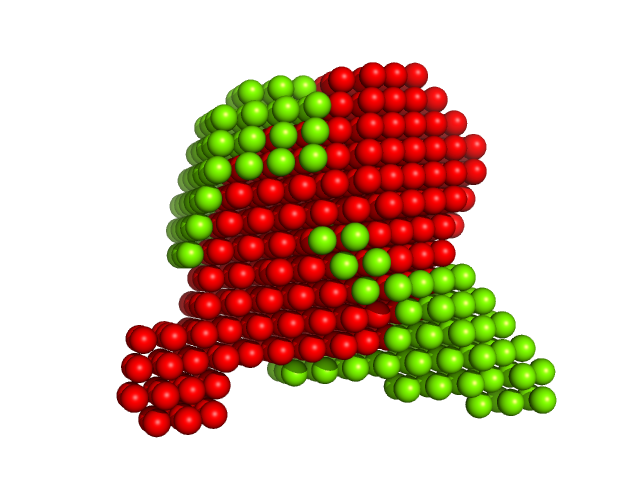
\includegraphics[scale=0.45]{initial.png}
\caption{two DAM before any movement ($NSD = 1.01$)}
\label{fgr:initial}
\end{figure}

\begin{figure}
\centering
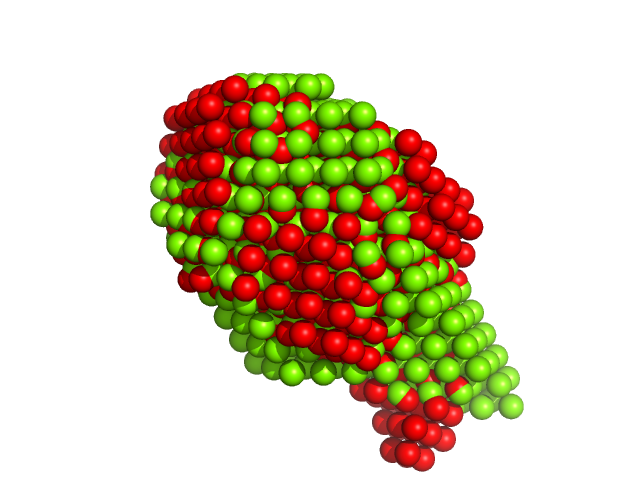
\includegraphics[scale=0.45]{rotated.png}
\caption{two DAM after canonical translation and rotation ($NSD = 0.60$)}
\label{fgr:rotated}
\end{figure}

\begin{figure}
\centering
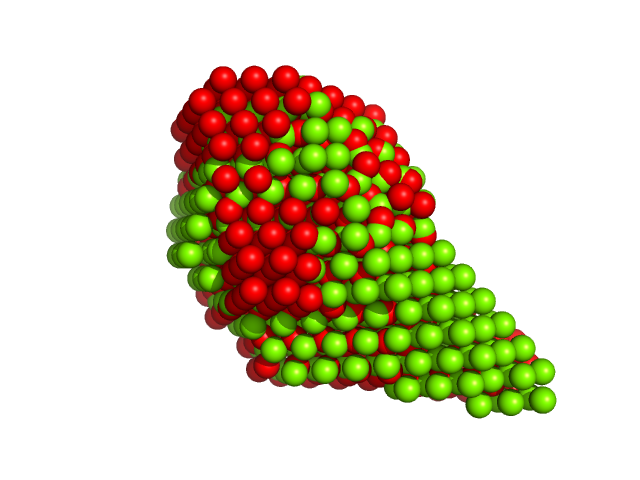
\includegraphics[scale=0.45]{symmetry.png}
\caption{two DAM after canonical translation and rotation and the 
  selection of an enantiomorph ($NSD = 0.58$)}
\label{fgr:symmetry}
\end{figure}

\begin{figure}
\centering
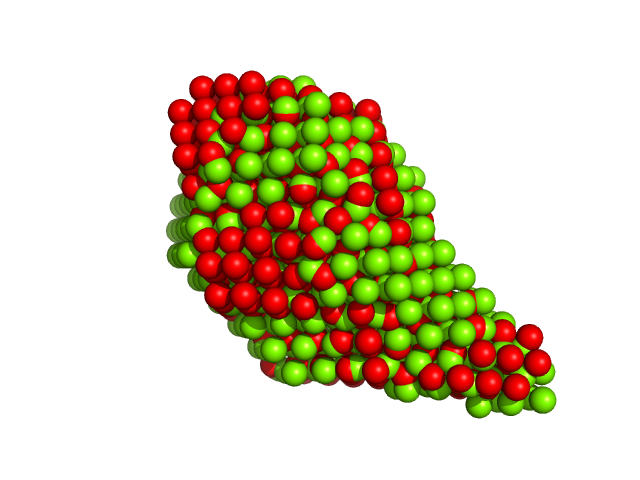
\includegraphics[scale=0.45]{superimposed.png}
\caption{two DAM after a refined superimposition ($NSD = 0.51$)}
\label{fgr:refined}
\end{figure}

\chapter{Performances comparison}
\label{perfappendix}

Some tests have been performed to compare in the same situations the 
different execution times of both \textsc{atsas}' supcomb and FreeSAS' 
SuPyComb. 
These execution times have been computed with Scisoft12, a computer 
fitted with two processors Intel(R) Xeon(R) CPU E5-2667 0 @ 2.90GHz, 
six cores each.

Data used as inputs are pdb files from dammif, computed from the 
scattering curve of lysozyme, and with its two modes: fast and slow. 
With the first one, we have obtained 16 models of nearly 515 dummy 
atoms each; and with the second one, 16 models of nearly 3050 dummy 
atoms. 
Supcomb and SuPyComb are tested with four combinations of two options: 
\begin{itemize}
\item fast mode - enantiomorphs not allowed
\item fast mode - enantiomorphs allowed
\item slow mode - enantiomorphs not allowed
\item slow mode - enantiomorphs allowed
\end{itemize}

Results from dammif models in fast mode are presented in 
figure~\ref{fgr:perfdamfast} and those from dammif models in slow mode 
in figure~\ref{fgr:perfdamslow}. 
It clearly appears that SuPyComb presents advantages in terms of 
execution time, even if it is doing other thing that supcomb 
($R-value$ selection, figures plotting).

\begin{figure}
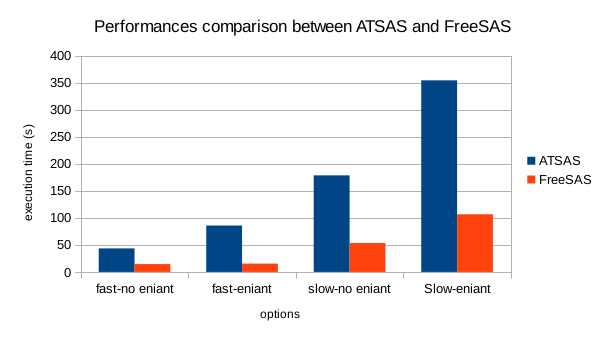
\includegraphics[scale=0.8]{perfdamfast.png}
\caption{Execution time of supcomb and SuPyComb with several option 
  for dammif fast mode (515 dummy atoms)}
\label{fgr:perfdamfast}
\end{figure} \vfill
\begin{figure}
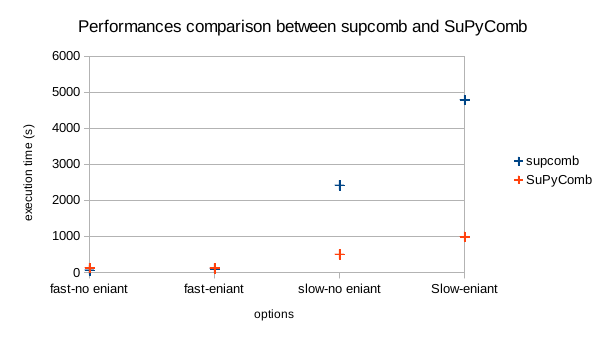
\includegraphics[scale=0.8]{perfdamslow.png}
\caption{Execution time of supcomb and SuPyComb with several option 
  for dammif slow mode (3050 dummy atoms)}
\label{fgr:perfdamslow}
\end{figure}

\end{document}

